\section{Materials and Methods}
\label{sec:methods}

\subsection{Open spectral and materials-property resources}
\label{subsec:data_sources}

Spec2Prop-InorgBench was constructed by integrating open spectral, crystallographic, and materials-property resources relevant to inorganic materials screening. Raman spectra were used as the primary spectral modality because they encode vibrational information associated with local bonding environments, anionic groups, lattice modes, hydration, and structural disorder. X-ray diffraction (XRD) patterns were used as an optional complementary modality because diffraction peak positions and intensities encode crystallographic and phase-level information. The RRUFF database provided the main Raman spectral backbone and available XRD links for mineral samples \cite{lafuente2015rruff,downs2006rruff}. Crystallographic context and phase-related motivation were supported by open crystallographic resources and recent XRD machine-learning benchmarks \cite{grazulis2009cod,grazulis2012cod,rincon2025simpod,guo2024xrddeeplearning}. Materials-property labels were linked using Materials Project and Matbench-derived annotations, including band-gap class, metal/non-metal class, and formation-energy class \cite{jain2013materialsproject,dunn2020matbench,riebesell2025matbenchdiscovery}. Table~\ref{tab:data_sources} summarizes the role of each data source.

\begin{table*}[htbp]
\centering
\caption{Open spectral, crystallographic, and materials-property resources used for constructing Spec2Prop-InorgBench.}
\label{tab:data_sources}
\small
\renewcommand{\arraystretch}{1.18}
\begin{tabularx}{\textwidth}{p{0.16\textwidth} p{0.14\textwidth} p{0.22\textwidth} p{0.14\textwidth} X p{0.11\textwidth}}
\toprule
\textbf{Source} & \textbf{Data type} & \textbf{Main fields used} & \textbf{Linkage key} & \textbf{Role in benchmark} & \textbf{Status} \
\midrule
RRUFF Raman \cite{lafuente2015rruff,downs2006rruff}
& Raman spectra
& Raman shift, intensity, raw spectral files, sample metadata
& RRUFF ID / sample ID
& Primary spectral backbone for Raman-based inorganic family screening and feature extraction
& Integrated \

RRUFF XRD \cite{lafuente2015rruff,downs2006rruff}
& Powder XRD patterns
& $2\theta$ values, diffraction intensities, linked sample records
& RRUFF ID / sample ID
& Optional multimodal branch for combining vibrational and crystallographic fingerprints
& Integrated \

RRUFF metadata \cite{lafuente2015rruff}
& Mineral chemistry
& Mineral name, chemical formula, sample identifier, chemistry notes
& RRUFF ID / formula
& Formula normalization and inorganic chemical-family label construction
& Integrated \

Materials Project \cite{jain2013materialsproject}
& Computed materials properties
& Band gap, formation energy, metallicity-related information, reduced formula
& Normalized reduced formula
& Source of materials-property annotations used for spectra-to-property classification
& Integrated \

Matbench \cite{dunn2020matbench,riebesell2025matbenchdiscovery}
& Benchmark property labels
& Band-gap class, metal/non-metal class, formation-energy-related labels
& Normalized reduced formula
& Standardized property-label source for downstream materials-informatics tasks
& Integrated \

MLROD
& Auxiliary Raman/mineral resource
& Raman/mineral records and mixture-related information
& Dataset-specific sample identifiers
& Auxiliary reference for robustness analysis and future extension; not used as the primary sample-level backbone
& Auxiliary \

tmQM/tmQMg
& Coordination-chemistry datasets
& Transition-metal complex formulas and molecular/property metadata
& Formula / complex identifier
& Context resource for future transition-metal and coordination-chemistry expansion; not used as primary Raman/XRD training data
& Auxiliary \

Spec2Prop-InorgBench \cite{kumar2026spec2prop}
& Curated benchmark
& Cleaned Raman/XRD representations, family labels, property labels, split metadata
& Internal sample ID
& Final released benchmark for reproducible inorganic spectra-to-property screening
& Released \
\bottomrule
\end{tabularx}
\end{table*}


\subsection{Construction of Spec2Prop-InorgBench}
\label{subsec:dataset_construction}

The benchmark was built through a multi-stage curation workflow designed to connect raw spectral files with chemically meaningful labels and downstream materials-property annotations. First, raw Raman records were collected and standardized at the sample level. Samples with unusable spectral files, missing essential metadata, or non-inorganic chemistry were removed. Chemical formulas were normalized to reduce inconsistencies caused by formatting differences, hydration notation, mixed occupancy, charge notation, or mineral-name duplication. Where possible, Raman records were linked to XRD patterns through shared mineral/sample identifiers. Property labels were then assigned by matching normalized reduced formulas to Materials Project/Matbench-derived entries.

This curation process produced four reportable benchmark subsets. The full spectral subset contains 4,118 usable Raman spectra. After inorganic filtering and chemical-label harmonization, the clean inorganic subset contains 4,027 samples and serves as the main dataset for chemical-family classification. The property-matched subset contains 1,844 samples with usable materials-property labels. The Raman--XRD linked subset contains 1,462 samples with both Raman and XRD representations and is used for multimodal analysis. The dataset construction funnel is shown in Figure~\ref{fig:funnel}, and subset definitions are summarized in Table~\ref{tab:dataset_subsets}.

\begin{figure}[!ht]
\centering
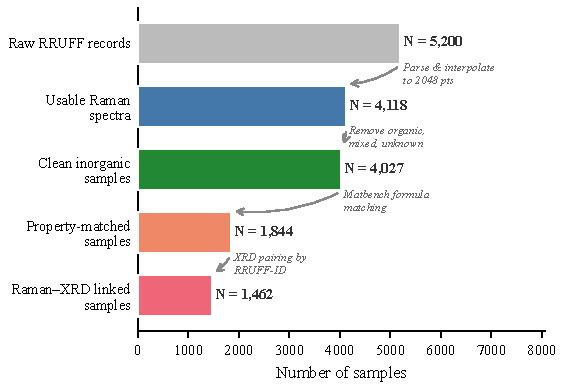
\includegraphics[width=\linewidth]{figures/fig2_dataset_funnel.pdf}
\caption{Dataset construction funnel for Spec2Prop-InorgBench. Raw open spectral records were filtered and harmonized to obtain 4,118 usable Raman spectra, 4,027 clean inorganic samples, 1,844 property-matched samples, and 1,462 Raman--XRD linked samples.}
\label{fig:funnel}
\end{figure}

\begin{table}[htbp]
\caption{Dataset subset statistics for Spec2Prop-InorgBench}
\label{tab:dataset_subsets}
\centering
\begin{tabularx}{\textwidth}{l c c c c X}
\toprule
\textbf{Subset} & \textbf{Samples} & \textbf{Raman} & \textbf{XRD} & \textbf{Property labels} & \textbf{Main use} \\
\midrule
Full spectra & 4,118 & Yes & Partial & Partial & Pretraining, exploration \\
Clean inorganic & 4,027 & Yes & Partial & Partial & Family classification \\
Property-matched & 1,844 & Yes & Partial & Yes & Spectra-to-property \\
Raman--XRD linked & 1,462 & Yes & Yes & Partial & Multimodal fusion \\
\bottomrule
\end{tabularx}
\end{table}


\subsection{Inorganic chemical-family label construction}
\label{subsec:family_labels}

Chemical-family labels were constructed from normalized chemical formulas and mineral metadata. The original chemistry labels were first organized into twelve inorganic groups, including silicates, oxides, sulfates, phosphates, sulfides, halides, carbonates, borates, elemental/native phases, telluride/selenide phases, intermetallic/alloy phases, and carbides. For model-level classification, rare or low-support groups were merged into an \textit{Other/Rare} category to reduce label sparsity and improve screening robustness. The final fine-grained model uses nine families: Borate, Carbonate, Halide, Other/Rare, Oxide, Phosphate, Silicate, Sulfate, and Sulfide.

This family-label design is chemically motivated. Silicates are dominated by Si--O framework and tetrahedral vibration modes; carbonates and phosphates contain characteristic anionic-group vibrations; oxides often show metal--oxygen lattice modes; sulfides and halides may exhibit lower-frequency or sparse Raman features; and borates contain B--O vibrational signatures. The \textit{Other/Rare} class captures chemically valid but underrepresented groups that cannot support reliable independent model training. Table~\ref{tab:family_defs} defines the final chemical-family labels used in this study.

\begin{table}[htbp]
\caption{Inorganic chemical family definitions and spectral relevance}
\label{tab:family_defs}
\centering

\begin{tabular}{llll}
\toprule
\textbf{Family} & \textbf{Chemical meaning} & \textbf{Representative spectral features} & \textbf{Model role} \\
\midrule
Silicate & Contains [SiO$_4$]$^{4-}$ units & Strong Si--O stretching (800--1200 cm$^{-1}$) & Target Class \\
Oxide & Contains O$^{2-}$ with metals & M--O vibrations (broad, variable) & Target Class \\
Carbonate & Contains [CO$_3$]$^{2-}$ units & Sharp C--O symmetric stretch ($\sim$1090 cm$^{-1}$) & Target Class \\
Sulfate & Contains [SO$_4$]$^{2-}$ units & Sharp S--O symmetric stretch ($\sim$980--1010 cm$^{-1}$) & Target Class \\
Phosphate & Contains [PO$_4$]$^{3-}$ units & P--O symmetric stretch ($\sim$960 cm$^{-1}$) & Target Class \\
Sulfide & Contains S$^{2-}$ with metals & Low wavenumber M--S modes ($<$500 cm$^{-1}$) & Target Class \\
Halide & Contains F$^-$, Cl$^-$, Br$^-$, I$^-$ & Very low wavenumber lattice modes & Target Class \\
Borate & Contains [BO$_3$]$^{3-}$/[BO$_4$]$^{5-}$ & B--O stretching ($\sim$1300--1500 cm$^{-1}$) & Target Class \\
Other/Rare & Nitrates, tungstates, etc. & Varies & Target Class \\
\bottomrule
\end{tabular}

\end{table}


\subsection{Runtime Raman and XRD spectral preprocessing}
\label{subsec:preprocessing}

Raw Raman and XRD files are not directly suitable for machine-learning inference because different instruments and databases may use different sampling grids, axis ranges, intensity scales, and file formats. Therefore, we implemented a runtime preprocessing pipeline that converts raw instrument-style spectra into fixed-length model-ready arrays. Raman spectra were standardized over the 100--4000~cm$^{-1}$ range, while XRD patterns were standardized over the 5--90$^\circ$ $2\theta$ range. Each spectrum was parsed into an axis--intensity representation, cleaned to remove invalid rows, sorted by spectral axis, deduplicated where repeated axis values occurred, interpolated to a fixed 2048-point grid, baseline-corrected, smoothed, and normalized.

\begin{figure}[!ht]
\centering
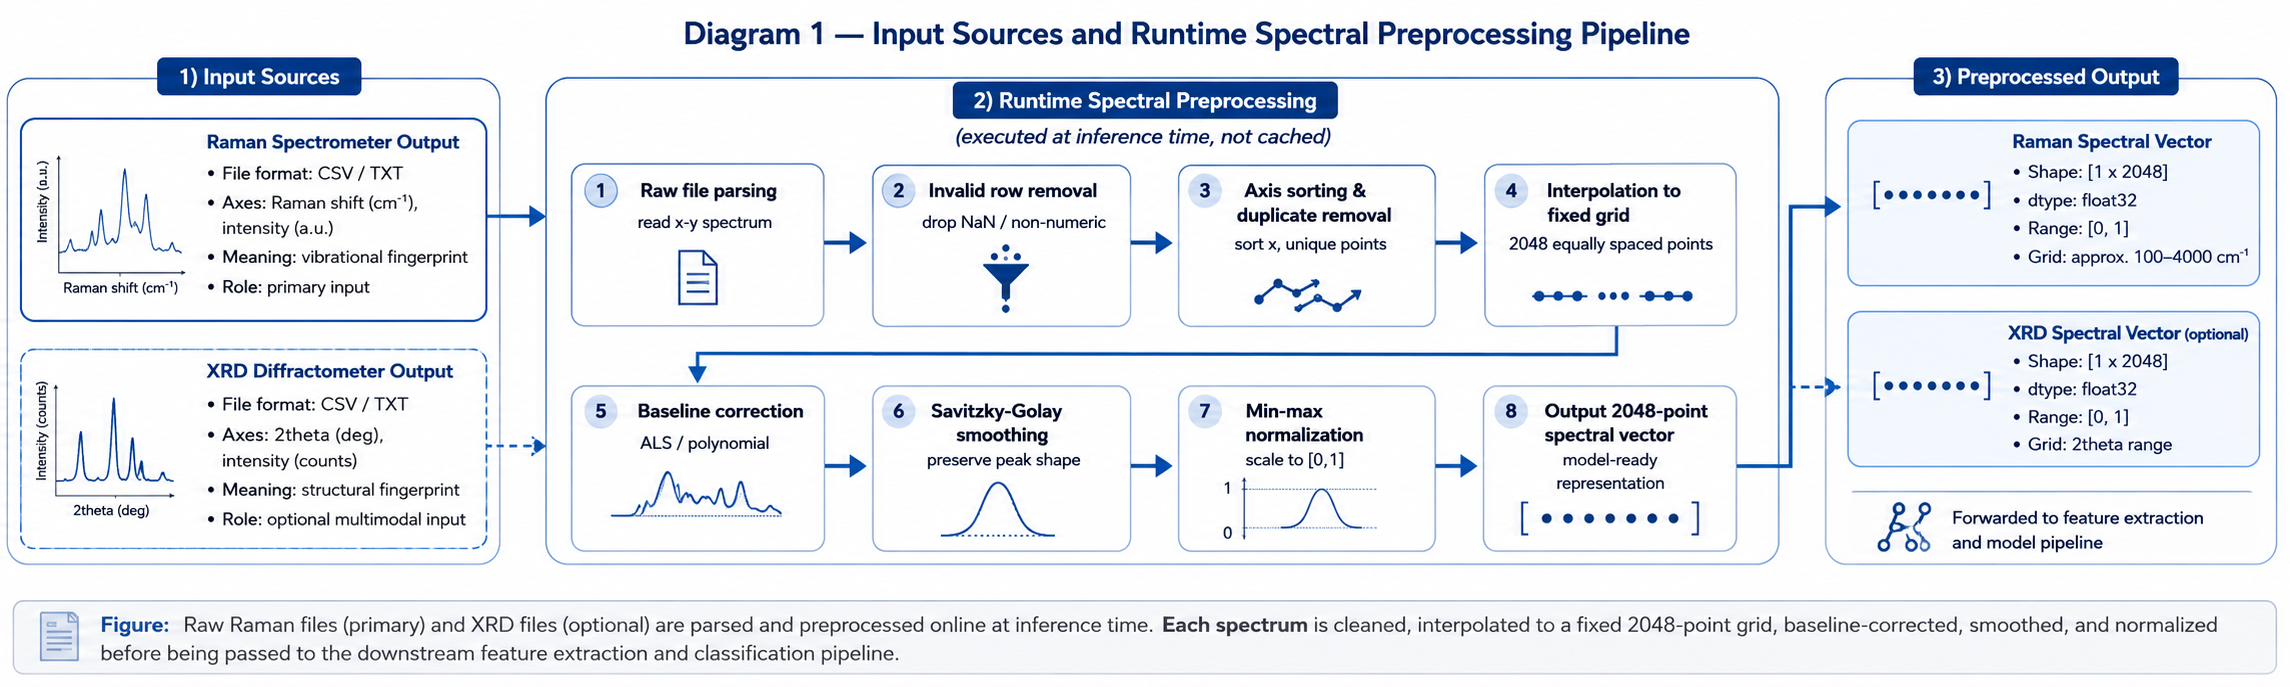
\includegraphics[width=\linewidth]{figures/preprocessing.png}
\caption{Runtime Raman/XRD spectral preprocessing pipeline. Raw spectral files are parsed, cleaned, axis-sorted, deduplicated, interpolated to a 2048-point grid, baseline-corrected, smoothed, normalized, and converted into model-ready spectral vectors.}
\label{fig:preprocessing}
\end{figure}

Baseline correction was used to reduce slowly varying fluorescence or background effects in Raman spectra \cite{zhang2010airpls,baek2015arpls}. Savitzky--Golay smoothing was applied with a window length of 11 and polynomial order of 3 to suppress high-frequency noise while preserving local peak structure \cite{savitzky1964smoothing}. Intensity normalization was performed after smoothing so that models learned relative spectral patterns rather than absolute intensity scale differences. The same fixed-length representation was used for Raman and optional XRD arrays, enabling both single-modality and multimodal experiments. The preprocessing sequence is summarized in Table~\ref{tab:preprocessing}.

\begin{table}[htbp]
\caption{Runtime preprocessing operations for raw Raman/XRD files}
\label{tab:preprocessing}
\centering

\begin{tabular}{llll}
\toprule
\textbf{Step} & \textbf{Operation} & \textbf{Chemistry/spectral reason} & \textbf{Output} \\
\midrule
1 & Raw file parsing & Instruments export heterogeneous text formats & Array of (X, Y) \\
2 & Invalid row removal & Cosmic rays and hardware errors yield NaNs & Cleaned array \\
3 & Axis sorting & Wavenumber axes can be reversed & Ascending X \\
4 & Duplicate removal & Multiple detector hits at same wavenumber & Unique X \\
5 & Interpolation & Align to uniform grid (e.g., 200--1500 cm$^{-1}$) & 2048-d vector \\
6 & Baseline correction & Remove fluorescence drift \cite{baek2015arpls} & Flattened vector \\
7 & Savitzky--Golay & Smooth high-frequency instrumental noise & Smoothed vector \\
8 & Min--Max normalization & Correct intensity variance across instruments & $[0, 1]$ scaled vector \\
\bottomrule
\end{tabular}

\end{table}


\subsection{Chemistry-aware spectral feature extraction}
\label{subsec:feature_extraction}

Instead of relying only on end-to-end black-box representations, we designed chemistry-aware spectral descriptors that explicitly encode peak, band-window, shape, and similarity information. The starting representation for each Raman sample is a 2048-point normalized intensity vector. From this vector, we extracted a base 158-dimensional PCA+domain representation consisting of 32 PCA global-shape features and 126 expert spectral descriptors. The expert descriptors include peak positions, peak heights, peak widths, spectral moments, diagnostic band-window intensities and ratios, derivative statistics, spectral entropy, integrated band areas, and compact subsampled spectral-shape features.

The diagnostic band-window descriptors were designed to capture chemically meaningful spectral regions associated with inorganic families. For example, silicate-related windows encode Si--O bending and stretching behavior; carbonate and phosphate windows target characteristic anionic-group vibrations; oxide windows represent lower-frequency metal--oxygen lattice contributions; and O--H related regions help capture hydrated or hydroxylated phases. These features make the representation more interpretable than a purely learned embedding and allow tree-based models to exploit sparse but chemically meaningful spectral cues.

For deployment-oriented screening, the base 158-dimensional feature vector was extended with prototype-similarity descriptors, producing a 222-dimensional PCA--domain--prototype representation. The prototype descriptors compare each held-out spectrum against training-set class prototypes and provide reference-like similarity information for top-$k$ screening. This 222-dimensional representation was used by the final Spec2Prop-Edge deployment model. Table~\ref{tab:feature_groups} summarizes the feature groups.

\begin{table}[htbp]
\caption{Chemistry-aware spectral feature groups}
\label{tab:feature_groups}
\centering
\begin{tabular}{lccl}
\toprule
\textbf{Feature group} & \textbf{Dimension} & \textbf{Used in final model} & \textbf{Chemical interpretation} \\
\midrule
PCA global-shape features & 32 & Yes & Broad spectral background and continuum \\
Expert descriptors & 126 & Yes & Specialized extraction of diagnostic peaks \\
\hspace{3mm} Peak statistics & 45 & Yes & Identification of primary vibrational modes \\
\hspace{3mm} Spectral moments & 30 & Yes & Overall spectral mass and skewness \\
\hspace{3mm} Diagnostic band ratios & 25 & Yes & Relative intensities of anion groups \\
\hspace{3mm} Compact shape features & 26 & Yes & Low-resolution baseline approximation \\
\midrule
Total vector & 158 & Yes & \\
\bottomrule
\end{tabular}
\end{table}


\begin{figure}[!ht]
\centering
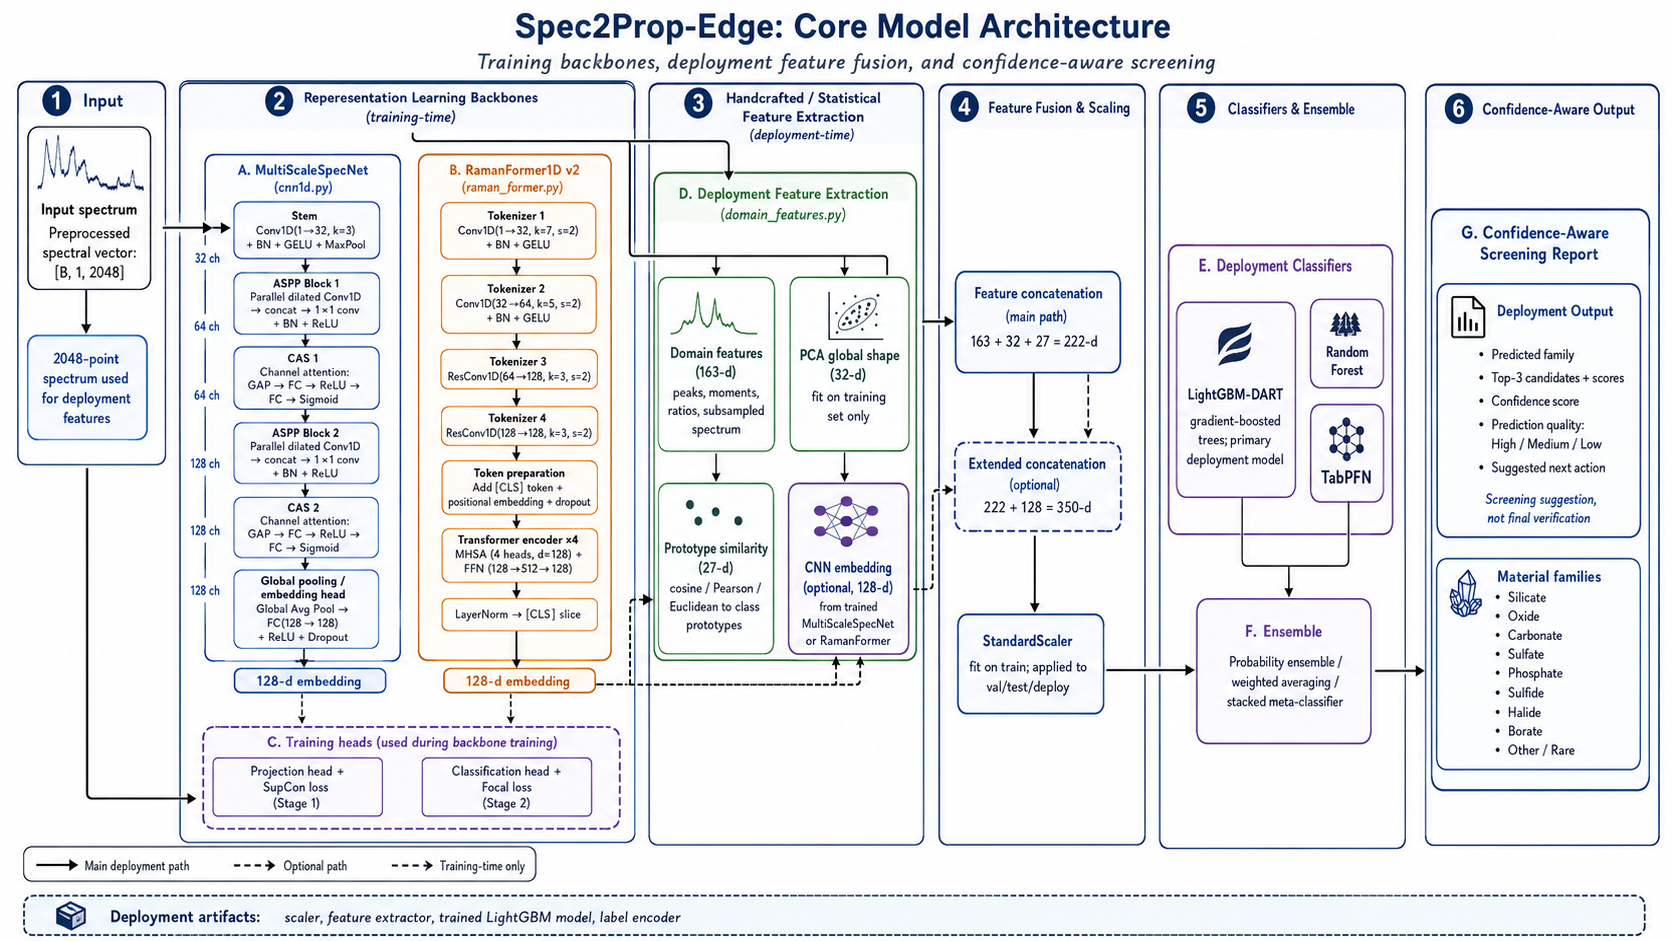
\includegraphics[width=\linewidth]{figures/model_architecture.png}
\caption{Feature extraction and LightGBM-DART screening architecture. The 2048-point Raman vector is transformed into PCA global-shape features, expert spectral descriptors, and prototype-similarity features. These are concatenated into a deployment-oriented 222-dimensional representation used by LightGBM-DART to predict top-$k$ inorganic chemical-family candidates and confidence scores.}
\label{fig:architecture}
\end{figure}

\subsection{Machine-learning models}
\label{subsec:ml_models}

The main deployment model is a LightGBM classifier using Dropout meets Multiple Additive Regression Trees (DART) boosting \cite{ke2017lightgbm,rashmi2015dart}. LightGBM-DART was selected because gradient-boosted decision trees are well suited for heterogeneous tabular spectral descriptors, handle nonlinear interactions between sparse peak features and global-shape features, and remain effective for small-to-moderate scientific datasets where purely end-to-end neural models may overfit. The DART boosting strategy randomly drops trees during training, reducing over-specialization and improving robustness \cite{rashmi2015dart}.

We benchmarked LightGBM-DART against classical and neural baselines. Classical baselines included Logistic Regression, support vector machines (SVM), k-nearest neighbors, Random Forest, XGBoost, and CatBoost \cite{cortes1995svm,chang2011libsvm,breiman2001randomforest,chen2016xgboost,dorogush2018catboost,pedregosa2011sklearn}. Neural baselines included SimpleCNN1D and RamanFormer1D for Raman-only family classification. For spectra-to-property prediction, we evaluated descriptor-only and fusion-based models, including DescriptorMLP, Spec2PropLite, and FusionSpec2PropNet. For multimodal Raman--XRD experiments, we evaluated a DualBranchRamanXRDNet that processes Raman and XRD vectors through separate branches before feature fusion. Model configurations are summarized in Table~\ref{tab:models}.

\begin{table*}[htbp]
\centering
\caption{Machine-learning model configurations used in Spec2Prop-InorgBench.}
\label{tab:models}
\footnotesize
\renewcommand{\arraystretch}{1.18}
\begin{tabularx}{\textwidth}{p{0.18\textwidth} p{0.21\textwidth} p{0.16\textwidth} p{0.19\textwidth} X}
\toprule
\textbf{Model} & \textbf{Input representation} & \textbf{Output task} & \textbf{Purpose} & \textbf{Key settings / notes} \
\midrule

Logistic Regression
& Raw Raman or PCA-reduced Raman features
& 9-class family classification
& Linear baseline
& Used to evaluate whether family separation is approximately linear in raw/PCA spectral space; L2 regularization used. \

SVM
& PCA-reduced Raman features and raw Raman ablation
& 9-class family classification
& Nonlinear baseline
& RBF-kernel SVM baseline for nonlinear decision boundaries in spectral feature space. \

kNN
& PCA-reduced Raman features and raw Raman ablation
& 9-class family classification
& Instance-based baseline
& Used as a simple spectral-neighbourhood baseline to test whether local similarity alone is sufficient for family screening. \

Random Forest
& PCA/domain spectral features
& 9-class family classification and property baselines
& Tree-ensemble baseline
& Used to evaluate the strength of non-boosted tree ensembles on sparse spectral descriptors and PCA features. \

XGBoost
& PCA/domain spectral features; raw and descriptor-only ablations
& Family classification and property baselines
& Gradient-boosted tree baseline
& Main boosted-tree comparison model. Hybrid experiments used up to 1000 estimators, maximum depth 6, and early stopping where applicable. \

LightGBM-DART, PCA+Domain ablation
& 158-d feature vector: 32 PCA features + 126 domain descriptors
& 9-class family classification
& Compact ablation model
& DART boosting with balanced class weights. This compact feature setting achieved the strongest top-1 accuracy among PCA+domain-only models and is reported as an ablation. \

LightGBM-DART, PCA+Domain+Prototype
& 222-d feature vector: PCA features + domain descriptors + prototype-similarity features
& 9-class family classification with top-$k$ confidence reporting
& Final Spec2Prop-Edge deployment model
& Deployment-oriented classifier using DART boosting, 1000 estimators, maximum depth 6, and balanced class weights. This model supports top-$k$ prediction, confidence scoring, and reject-option screening. \

SimpleCNN1D
& 2048-point Raman vector
& Family classification and property baseline
& End-to-end neural baseline
& One-dimensional convolutional baseline trained directly on Raman spectra. Used to compare learned spectral features against chemistry-aware descriptors. \

LiteSpecNet / Spec2PropLite
& 2048-point Raman vector + descriptor features
& Spectra-to-property prediction
& Edge-friendly fusion model
& Lightweight Raman encoder combined with descriptor features. Used for property prediction, especially metal/non-metal classification. \

RamanFormer1D
& 2048-point Raman vector
& Family classification
& Transformer-based neural baseline
& Spectral transformer baseline used to test whether attention-based sequence modelling improves Raman family classification. \

DescriptorMLP
& Chemistry/domain descriptor vector
& Spectra-to-property prediction
& Descriptor-only neural baseline
& Multi-layer perceptron trained on descriptor features only; used to test how much property information is captured by engineered descriptors. \

FusionSpec2PropNet
& Raman CNN embedding + descriptor embedding
& Multi-task property prediction
& Raman--descriptor fusion model
& Combines a Raman CNN encoder and DescriptorMLP encoder, concatenates embeddings, applies a fusion layer, and predicts band-gap class, metal/non-metal class, and formation-energy class. \

DualBranchRamanXRDNet
& Raman vector + XRD vector, each 2048 points
& 9-class family classification
& Multimodal Raman--XRD baseline
& Dual-branch neural model with separate Raman and XRD encoders followed by feature fusion. Used to evaluate complementarity between vibrational and crystallographic fingerprints. \

\bottomrule
\end{tabularx}
\end{table*}


\subsection{Leakage-safe evaluation protocol}
\label{subsec:evaluation}

A leakage-safe evaluation protocol was used to reduce overoptimistic performance caused by duplicated spectra, repeated measurements, or closely related entries appearing across train and test sets. The dataset was split into 70% training, 15% validation, and 15% test partitions. Splitting was grouped by RRUFF identifier and stratified by chemical family and band-gap class where applicable. This strategy reduces the risk that highly similar measurements of the same sample or mineral record appear in both training and test partitions.

All preprocessing parameters, PCA transformations, class prototypes, and feature scalers were fitted only on the training split and then applied to validation and test splits. Family classification was evaluated using accuracy, macro-F1, weighted-F1, balanced accuracy, and top-$k$ accuracy. Macro-F1 was emphasized because the nine-family classification task is class-imbalanced. Property prediction was evaluated separately for band-gap class, metal/non-metal classification, and formation-energy class. Confidence-aware screening was evaluated by measuring accuracy and macro-F1 at different acceptance thresholds, where low-confidence predictions were abstained rather than forced into a final class. The complete evaluation design is summarized in Table~\ref{tab:protocol}.
\subsection{Mathematical formulation of spectral preprocessing}
\label{subsec:preprocessing_formulas}

Let a raw Raman or XRD spectrum be represented as a set of axis--intensity pairs,
\begin{equation}
S_{\mathrm{raw}}={(x_i,y_i)}_{i=1}^{M},
\end{equation}
where $x_i$ denotes the Raman shift in cm$^{-1}$ for Raman spectra or the diffraction angle $2\theta$ in degrees for XRD patterns, and $y_i$ is the corresponding measured intensity. The number of raw points $M$ may vary across files because of differences in instruments, acquisition settings, or database formats. Therefore, the first objective of preprocessing is to transform each variable-length spectrum into a fixed-length model-ready vector.

Invalid entries were removed by retaining only finite axis and intensity values:
\begin{equation}
S_{\mathrm{clean}}={(x_i,y_i): x_i \in \mathbb{R},, y_i \in \mathbb{R},, \mathrm{isfinite}(x_i),, \mathrm{isfinite}(y_i)}.
\end{equation}
This step prevents missing values, corrupted rows, or non-numeric entries from propagating into interpolation and machine-learning inference.

The cleaned spectra were sorted by the spectral axis, and duplicate axis values were merged by averaging their intensities:
\begin{equation}
\bar{y}(x)=\frac{1}{|\mathcal{I}(x)|}\sum_{i\in \mathcal{I}(x)}y_i,
\end{equation}
where $\mathcal{I}(x)={i:x_i=x}$ is the set of repeated measurements at the same spectral coordinate. This avoids unstable interpolation caused by duplicated $x$ values.

Each spectrum was then interpolated onto a fixed grid of $N=2048$ points. For Raman spectra, the grid was defined over $[100,4000]$ cm$^{-1}$, while for XRD spectra it was defined over $[5,90]^\circ$ $2\theta$:
\begin{equation}
x_j^{*}=x_{\min}+\frac{j}{N-1}(x_{\max}-x_{\min}), \qquad j=0,1,\ldots,N-1.
\end{equation}
Linear interpolation was used to estimate the intensity at each grid point:
\begin{equation}
y^{*}(x_j^{*}) =
y_a+\frac{y_b-y_a}{x_b-x_a}(x_j^{*}-x_a),
\qquad x_a \leq x_j^{*} \leq x_b,
\end{equation}
where $(x_a,y_a)$ and $(x_b,y_b)$ are the nearest neighboring raw spectral points surrounding $x_j^{*}$. Interpolation makes spectra comparable across samples and ensures that all models receive inputs with identical dimensionality.

To reduce slowly varying fluorescence or background contributions, baseline correction was applied. The estimated baseline $b$ can be expressed as the solution of a penalized least-squares problem:
\begin{equation}
\hat{b}=\arg\min_{b}\left[
\sum_{j=1}^{N}w_j(y_j^{*}-b_j)^2
+\lambda|D^{(m)}b|_2^2
\right],
\end{equation}
where $w_j$ are adaptive weights, $\lambda$ controls baseline smoothness, and $D^{(m)}$ is an $m$th-order difference operator. The baseline-corrected spectrum is then
\begin{equation}
y_j^{\mathrm{bc}} = y_j^{*}-\hat{b}_j.
\end{equation}
This step is especially important for Raman spectra, where fluorescence background can obscure chemically meaningful peaks.

High-frequency noise was reduced using Savitzky--Golay smoothing. Around each point, a local polynomial of degree $p=3$ was fitted within a moving window of length $2h+1=11$:
\begin{equation}
\hat{y}^{\mathrm{bc}}(t)=\sum_{r=0}^{p}a_r t^r,
\end{equation}
and the smoothed value was taken at the center of the window:
\begin{equation}
y_j^{\mathrm{sg}}=\sum_{k=-h}^{h}c_k y_{j+k}^{\mathrm{bc}}.
\end{equation}
Here, $c_k$ are the Savitzky--Golay convolution coefficients. This smoothing operation suppresses random noise while preserving peak position, width, and shape better than simple moving-average smoothing.

Finally, each spectrum was intensity-normalized using maximum-intensity normalization:
\begin{equation}
y_j^{\mathrm{norm}}=
\frac{y_j^{\mathrm{sg}}}
{\max_{1\leq l\leq N}|y_l^{\mathrm{sg}}|+\epsilon},
\end{equation}
where $\epsilon$ is a small constant to avoid division by zero for nearly flat spectra. The final preprocessed spectral vector is
\begin{equation}
\mathbf{s}=
[y_1^{\mathrm{norm}},y_2^{\mathrm{norm}},\ldots,y_N^{\mathrm{norm}}]^\top
\in \mathbb{R}^{2048}.
\end{equation}
This normalization reduces the effect of arbitrary instrument-dependent intensity scaling and allows the model to focus on relative spectral shape and peak structure.

\subsection{Mathematical formulation of chemistry-aware spectral descriptors}
\label{subsec:feature_formulas}

From each normalized Raman vector $\mathbf{s}\in\mathbb{R}^{2048}$, we extracted chemically interpretable descriptors representing peak structure, spectral distribution, diagnostic band responses, and reference-like similarity.

Peak-based descriptors were obtained by identifying local maxima with sufficient prominence and spacing. For the $k$th selected peak at index $p_k$, the normalized peak position, peak height, and relative width were encoded as
\begin{equation}
f_{p,k}=\frac{p_k}{N}, \qquad
f_{h,k}=s_{p_k}, \qquad
f_{w,k}=\frac{w_k}{N},
\end{equation}
where $N=2048$ and $w_k$ is the full width at half maximum estimated from the local peak profile. Peak descriptors are chemically useful because inorganic families often exhibit characteristic Raman bands associated with Si--O, M--O, CO$_3^{2-}$, PO$_4^{3-}$, SO$_4^{2-}$, B--O, O--H, or lattice vibration modes.

Global spectral moments were computed to summarize the intensity distribution:
\begin{equation}
\mu=\frac{1}{N}\sum_{j=1}^{N}s_j,
\end{equation}
\begin{equation}
\sigma=\sqrt{\frac{1}{N}\sum_{j=1}^{N}(s_j-\mu)^2+\epsilon},
\end{equation}
\begin{equation}
\mathrm{Skew}=\frac{1}{N}\sum_{j=1}^{N}\left(\frac{s_j-\mu}{\sigma}\right)^3,
\end{equation}
\begin{equation}
\mathrm{Kurt}=\frac{1}{N}\sum_{j=1}^{N}\left(\frac{s_j-\mu}{\sigma}\right)^4.
\end{equation}
These moments capture overall spectral sharpness, asymmetry, and intensity concentration, which are useful for distinguishing sharp crystalline spectra from broader or noisier patterns.

For each diagnostic Raman window $B_m=[l_m,u_m]$, the mean band intensity and integrated band area were computed as
\begin{equation}
\bar{s}*{B_m}=
\frac{1}{|B_m|}\sum*{j\in B_m}s_j,
\end{equation}
\begin{equation}
A_{B_m}=
\sum_{j\in B_m}s_j\Delta x.
\end{equation}
Band-ratio descriptors were then defined as
\begin{equation}
R_{m,n}=
\frac{\bar{s}*{B_m}+\epsilon}
{\bar{s}*{B_n}+\epsilon}.
\end{equation}
These ratios are useful because relative intensity across chemically meaningful spectral windows can be more robust than absolute intensity. For example, silicate, carbonate, phosphate, sulfate, oxide, and hydrated phases can show different relative responses across characteristic Raman regions.

A compact spectral-shape descriptor was obtained by subsampling the normalized spectrum with stride $q=32$:
\begin{equation}
\mathbf{s}*{\mathrm{sub}}=
[s_1,s*{1+q},s_{1+2q},\ldots,s_{1+63q}]^\top
\in \mathbb{R}^{64}.
\end{equation}
This retains coarse spectral morphology while reducing dimensionality, making it useful for tree-based models.

Global spectral-shape information was additionally encoded using principal component analysis (PCA). Let $\boldsymbol{\mu}*{\mathrm{train}}$ be the training-set mean spectrum and $\mathbf{W}*{32}$ be the first 32 principal components fitted only on the training split. The PCA feature vector is
\begin{equation}
\mathbf{z}*{\mathrm{PCA}}=
\mathbf{W}*{32}^{\top}(\mathbf{s}-\boldsymbol{\mu}_{\mathrm{train}})
\in \mathbb{R}^{32}.
\end{equation}
Fitting PCA only on the training set avoids information leakage from validation or test samples.

For the final deployment model, prototype-similarity descriptors were added. For each chemical family $c$, a training-set prototype spectrum was computed as
\begin{equation}
\boldsymbol{\pi}_c=
\frac{1}{|\mathcal{T}*c|}
\sum*{i\in\mathcal{T}_c}\mathbf{s}_i,
\end{equation}
where $\mathcal{T}*c$ is the set of training samples belonging to class $c$. Cosine similarity between a test spectrum and each class prototype was then computed as
\begin{equation}
\mathrm{sim}*{c}(\mathbf{s},\boldsymbol{\pi}_c)=
\frac{\mathbf{s}^{\top}\boldsymbol{\pi}_c}
{|\mathbf{s}|_2|\boldsymbol{\pi}_c|_2+\epsilon}.
\end{equation}
Prototype similarity provides a reference-library-like signal that complements peak and band-window descriptors during top-$k$ candidate screening.

The final deployment feature vector is expressed as
\begin{equation}
\mathbf{x}*{\mathrm{deploy}}=
[\mathbf{z}*{\mathrm{PCA}};
\mathbf{x}*{\mathrm{domain}};
\mathbf{x}*{\mathrm{proto}}]
\in \mathbb{R}^{222},
\end{equation}
where $\mathbf{z}*{\mathrm{PCA}}\in\mathbb{R}^{32}$, $\mathbf{x}*{\mathrm{domain}}$ contains expert spectral descriptors, and $\mathbf{x}_{\mathrm{proto}}$ contains prototype-similarity features. This representation combines global spectral shape, chemically interpretable Raman descriptors, and reference-like class similarity for confidence-aware inorganic material screening.

\begin{table*}[htbp]
\centering
\caption{Leakage-safe evaluation protocol used for family classification, spectra-to-property prediction, multimodal analysis, and confidence-aware screening.}
\label{tab:protocol}
\footnotesize
\renewcommand{\arraystretch}{1.18}
\begin{tabularx}{\textwidth}{p{0.17\textwidth} p{0.18\textwidth} X p{0.20\textwidth} X}
\toprule
\textbf{Task} & \textbf{Dataset subset} & \textbf{Split strategy} & \textbf{Metrics} & \textbf{Leakage control} \\
\midrule

Inorganic family classification
& Clean inorganic subset ($N=4{,}027$)
& 70/15/15 train--validation--test split, grouped by RRUFF ID and stratified by chemical family
& Accuracy, macro-F1, weighted-F1, balanced accuracy, top-$k$ accuracy, confusion matrix
& Samples sharing the same RRUFF identifier were kept within the same split. PCA, scalers, prototypes, and model parameters were fitted only on the training split. \\

Spectra-to-property prediction
& Property-matched inorganic subset ($N=1{,}844$)
& 70/15/15 train--validation--test split, grouped by RRUFF ID and stratified where applicable by property class
& Accuracy, macro-F1, macro-precision, macro-recall, per-class F1
& Formula-derived property labels were matched before splitting; transformations and descriptor normalization were fitted using training data only. \\

Raman--XRD multimodal classification
& Raman--XRD linked inorganic subset ($N=1{,}462$)
& 70/15/15 train--validation--test split using the same grouped-split logic
& Accuracy, macro-F1, macro-precision, macro-recall, relative gain over Raman-only ablation
& Raman and XRD records linked to the same sample or RRUFF identifier were assigned to the same split to avoid paired-modality leakage. \\

Confidence-aware screening
& Held-out test set from the deployment model
& Final model evaluated only on the untouched test split
& Top-1/top-2/top-3/top-5 accuracy, confidence score, coverage, accepted-sample accuracy, accepted-sample macro-F1, abstention rate
& Confidence thresholds were applied after test-set prediction. Low-confidence spectra were abstained rather than forced into final identification. \\

External/demo evaluation
& Dataset-backed held-out samples
& Test samples selected only from leakage-safe held-out split
& Top-$k$ candidate families, confidence tier, screening recommendation
& Demo samples were not used for model fitting, scaler fitting, PCA fitting, or prototype construction. \\

\bottomrule
\end{tabularx}
\end{table*}


\subsection{Confidence-aware deployment workflow}
\label{subsec:deployment}

Spec2Prop-Edge was designed as a deployment-style screening workflow rather than a final material-identification system. During inference, a raw Raman spectrum is parsed and preprocessed at runtime, transformed into a fixed 2048-point vector, converted into the 222-dimensional PCA--domain--prototype representation, and passed to the trained LightGBM-DART model. The model returns the predicted family, top-$k$ candidate families, class probabilities, and a confidence score. Predictions are assigned to high-, medium-, or low-confidence tiers using predefined probability thresholds.

The confidence-aware design is important because spectral ambiguity, mixed phases, class imbalance, and instrument variation can produce uncertain predictions. Instead of forcing every sample into a single final class, Spec2Prop-Edge reports candidate families for scientist verification and can abstain on low-confidence samples. This makes the workflow suitable for early-stage candidate prioritization, batch triage, and preliminary material-family interpretation, while final confirmation remains dependent on expert spectroscopic analysis, crystallographic validation, and laboratory verification \cite{guo2017calibration}.
